% \documentclass{article}
% \usepackage[utf8]{inputenc}
% \usepackage{graphicx}
\graphicspath{ {./images/} }
%\usepackage{hyperref}

\title{Turner  CS600}
\author{James Turner}
\date{September 2022}

%\begin{document}

\maketitle
\newpage
\section{Old Stuff from Assignment 1}
My name is James Turner and I am an active-duty Army Chief Warrant Officer 3 (CW3).  I have served a total of 17 years with 12 years as a Cyber Electromagnetic Warfare (EW) Technician.  This job field is extremely challenging because the technology in the marketplace and capabilities used by our adversaries is constantly changing.  However, it also stimulates innovation and creative thinking and is rewarding when you are part of a team that finds solutions to complex problems.

Recently, I was accepted into the Army’s Advanced Civil School (ACS) program that allows me to attend school full-time and complete a Master’s degree while on active duty.  I have been accepted at UCCS in the Cybersecurity Master of Engineering program, and I am a first term student.  I chose to study cybersecurity because my job field is closely connected with wireless applications and wireless security, and I realized that there is significant job growth in the cybersecurity field.

One of the primary outcomes that I desire from the CS6000 course is to become a more proficient writer and researcher.   I already possess some research and writing skills through my professional military education and on the job experience.  However, military style of writing differs from academia in that the military focuses on a “bottom line up front” perspective and tends to leave details out of formal documents.  I also hope to achieve a greater array of methods that help me conduct more thorough and rigorous research.

Another goal I desire from this course is to enhance my critical thinking.  The military embraces and teaches critical thinking at all levels of leadership education, but I want to gain a greater ability to analyze and test information with scientific methods.  The preponderance of my degree plan and research will be analyzing other tests and scientific data, so I want to be prepared to understand and evaluate those results.  I will need to sharpen my ability to challenge assumptions of others, including myself so that I can become a better researcher.

\begin{figure}
    \centering
    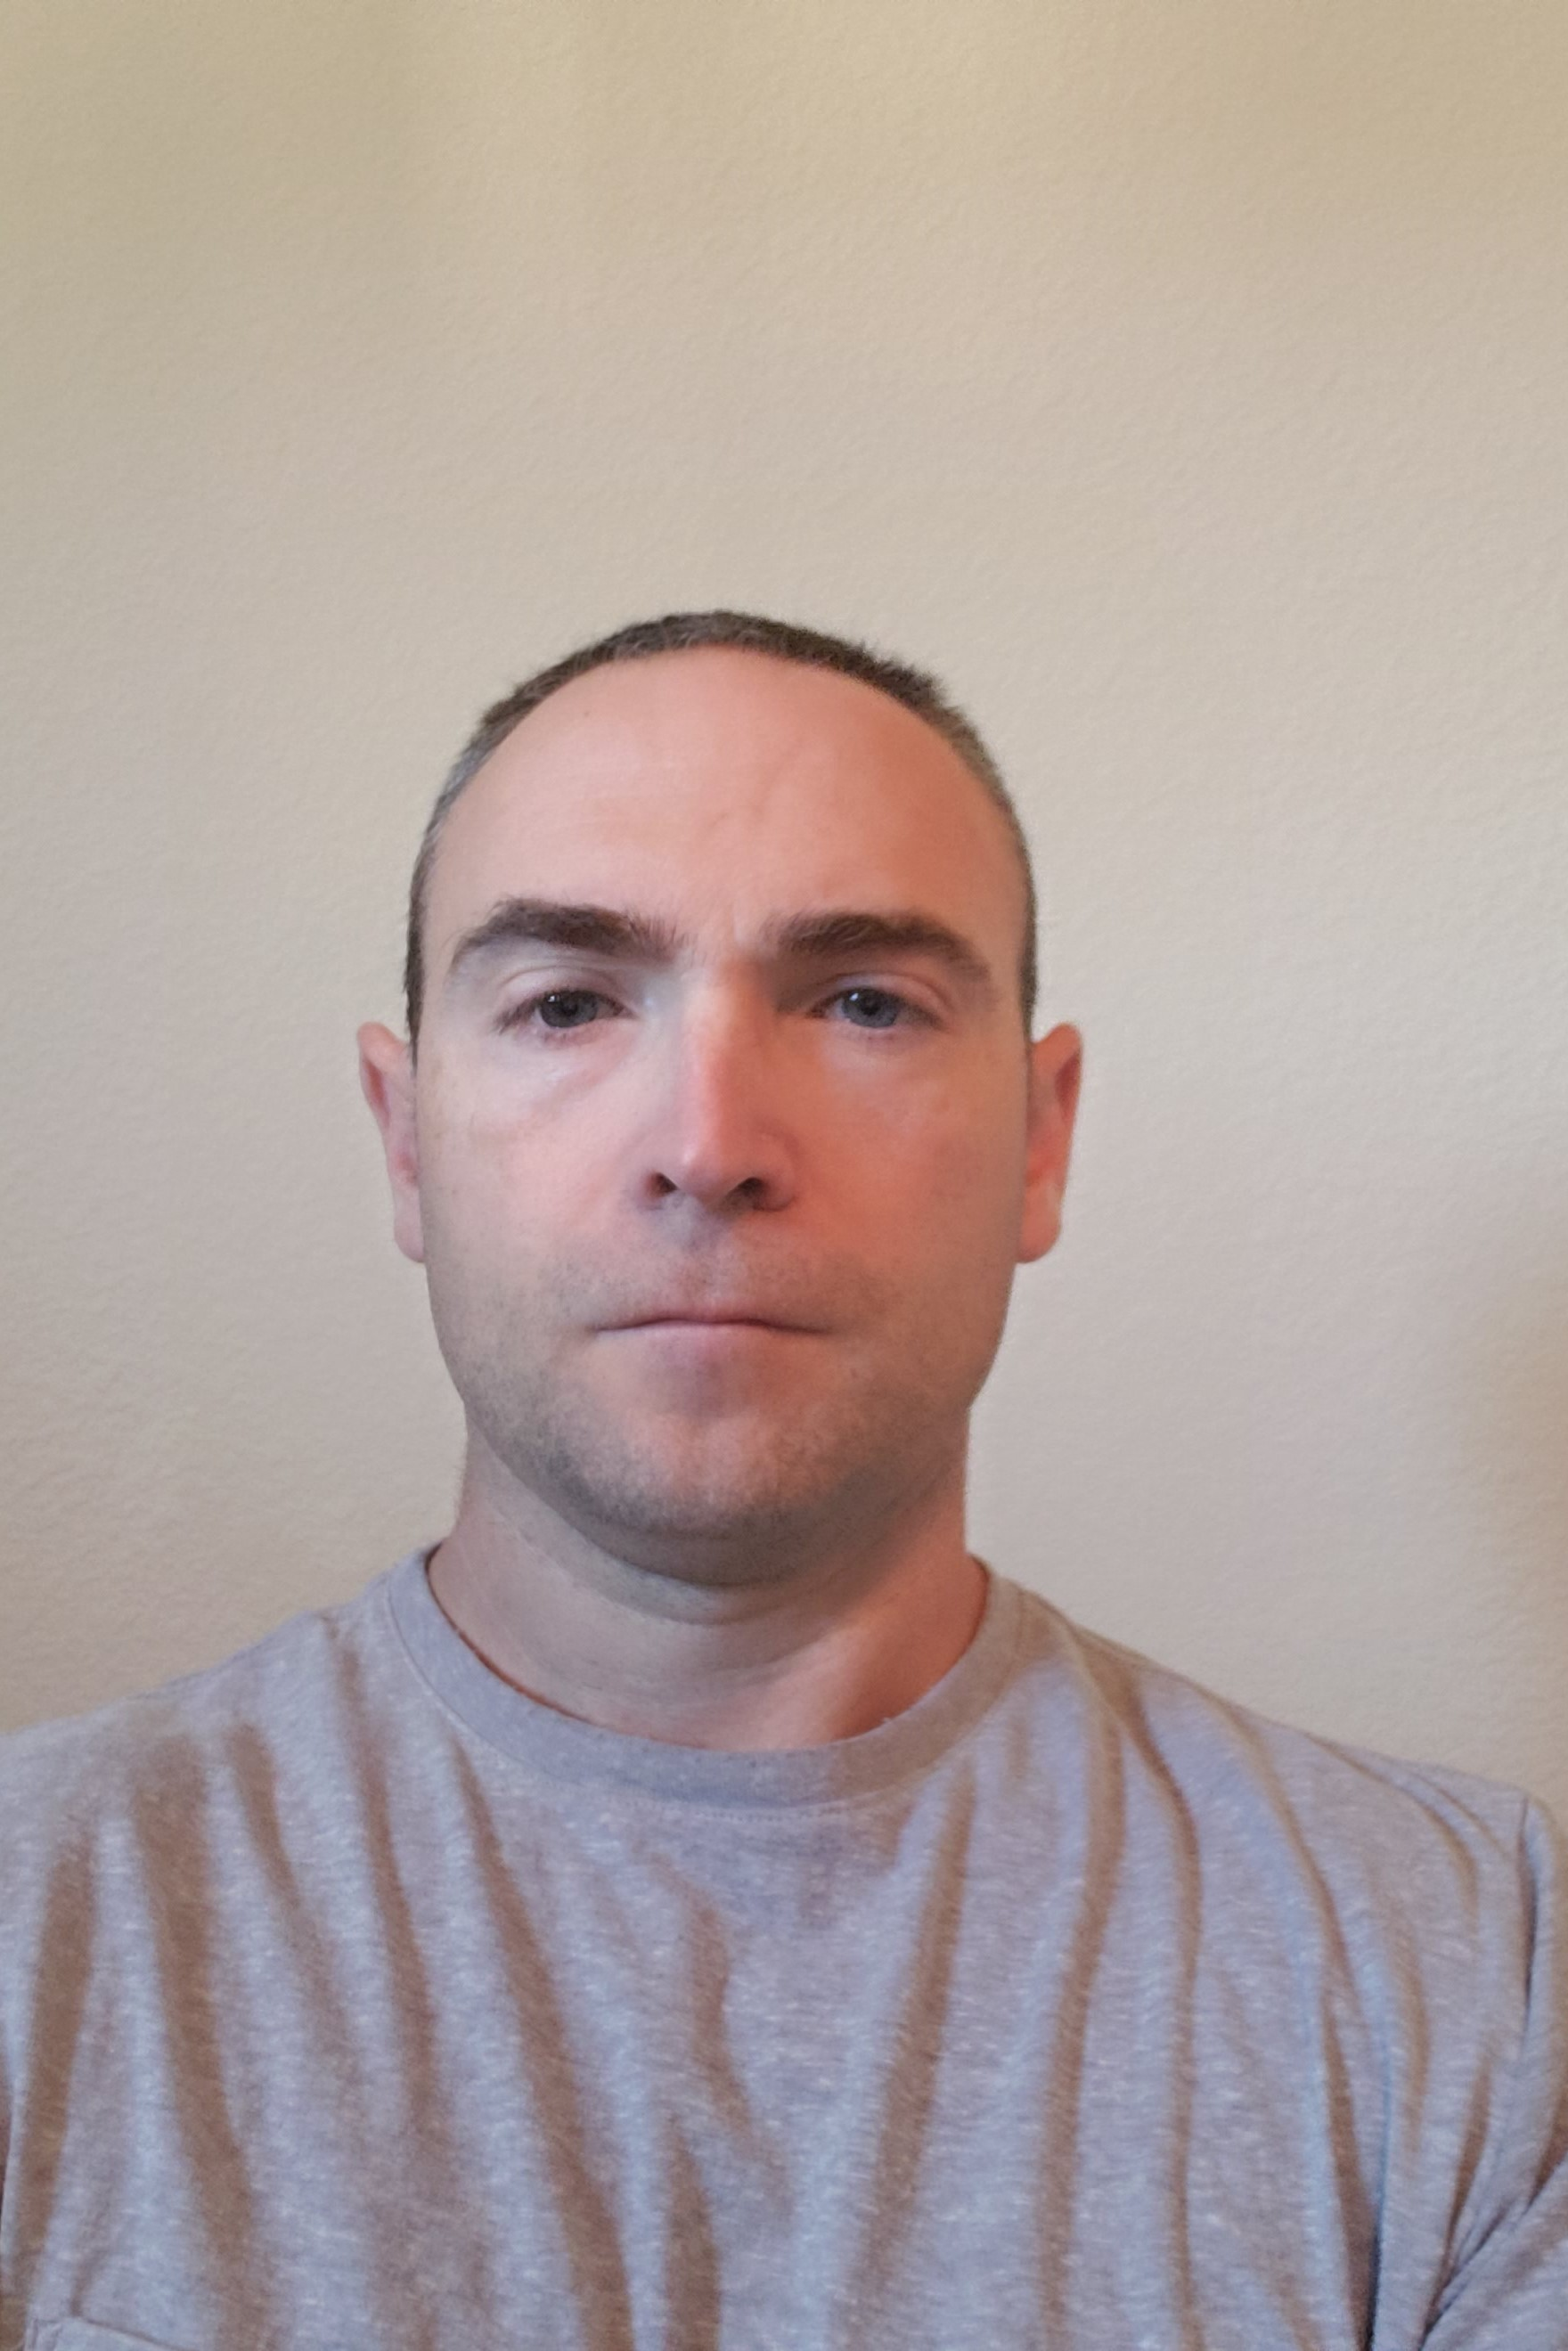
\includegraphics[scale=.1]{self pic2.jpg}
    \caption{me}
    \label{fig:me}
\end{figure}
%\newpage
\section{Github Code on Cognitive Radio}
This repository in Github contains a novel algorithm that uses linear processing to characterize the radio frequency environment in order to enable secondary users' ability to use unoccupied electromagnetic spectrum space.  The link is provided below.
\url{https://github.com/parthgargava/Cognitive-Radio-Networks}

\section{Questions}
What is the main topic that you like to work on for your master thesis, and how do you think that can benefit that army? Ali AlShami
\newline
\paragraph{}
Answer: If I still go the Thesis track then I will discuss some form of wireless security from an avaiability (redundancy and resiliency) and confidentiality perspective.  I still don't know what wireless application I will choose from.  I might focus on 5G or some new type of technology such as reconfigurable intelligent surfaces. 
\paragraph{}
Are you hoping to work on a theoretical or hands-on approach to electronic warfare? I imagine you get a fair share on hands-on experience already. -Katrina
Answer: If I can do live expirementation then that's what I will do.  Yes, I do have plenty of hands-on experiences with different forms of radios and their applications.  However, I need to get stronger from a theoretical standpoint as well.  When you play around with equipment, sometimes it's easy to lose track of the fundamentals in the design of that same equipment.

Nazmus: Have you used PKI in your research?

%\end{document}
